% Figure from MATH 591 notes, section 52. Compile with the notes preamble.
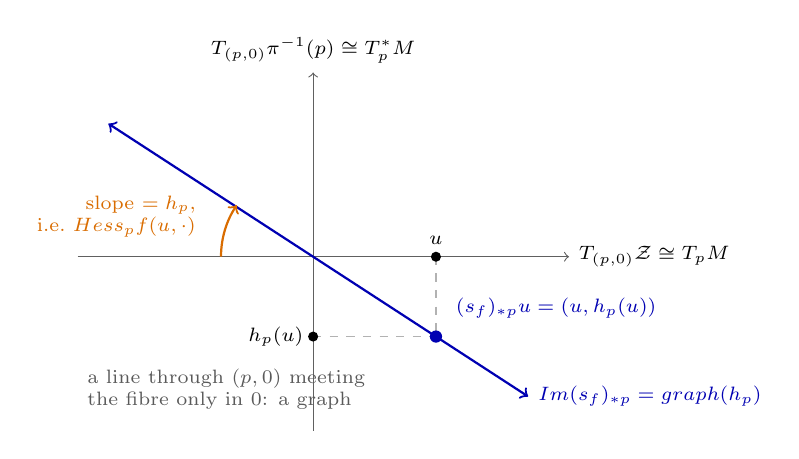
\begin{tikzpicture}[scale=1.3, font=\scriptsize]
\draw[->, gray!75!black] (-2.3,0) -- (2.5,0) node[right, text=black] {$T_{(p,0)}\mathcal{Z} \cong T_pM$};
\draw[->, gray!75!black] (0,-1.7) -- (0,1.8) node[above, text=black] {$T_{(p,0)}\pi^{-1}(p) \cong T_p^*M$};
\draw[<->, blue!70!black, thick] (-2.0,1.3) -- (2.1,-1.365) node[right] {$\operatorname{Im}(s_f)_{*p} = \operatorname{graph}(h_p)$};
\draw[gray!60, dashed] (1.2,0) -- (1.2,-0.78);
\draw[gray!60, dashed] (0,-0.78) -- (1.2,-0.78);
\fill (1.2,0) circle (1.4pt) node[above=1pt] {$u$};
\fill (0,-0.78) circle (1.4pt) node[left] {$h_p(u)$};
\fill[blue!70!black] (1.2,-0.78) circle (1.7pt);
\node[blue!70!black, anchor=west] at (1.3,-0.5) {$(s_f)_{*p}u = (u, h_p(u))$};
\draw[orange!85!black, thick, ->] (-0.9,0) arc (180:146:0.9);
\node[orange!85!black, anchor=south east, align=right] at (-1.05,0.1) {slope $= h_p$,\\ i.e.\ $\operatorname{Hess}_pf(u,\cdot)$};
\node[gray!70!black, anchor=north west, align=left] at (-2.3,-1.0) {a line through $(p,0)$ meeting\\ the fibre only in $0$: a graph};
\end{tikzpicture}
